
\documentclass[11pt,a4paper]{article}
\usepackage[left=2cm,right=2cm,top=2cm,bottom=3cm]{geometry}
\usepackage{amsmath,amsfonts,amsthm,amssymb,varioref,times, commath}
\usepackage{gensymb}
\usepackage{tikz}
\usepackage{textcomp}
\usepackage{hyperref}
\hypersetup{
 colorlinks=true,
 linkcolor=blue,
 filecolor=magenta, 
urlcolor=cyan,
}
\usepackage{lipsum}
\usepackage{epigraph}
%to resume numbering in a list
\usepackage{enumitem}
%----- arrows 
\usepackage{extarrows}

%    differential equatiosn 
\usepackage{diffcoeff}   %\diff[2]{x}{y}


%%%%%%pour ecrire en français avec les accents
\usepackage[utf8]{inputenc}
\usepackage[T1]{fontenc}
\usepackage{lmodern} % load a font with all the characters
\usepackage{units}
%%%%%%%Image-related packages
\usepackage{wrapfig}
\usepackage{float, graphicx}
\graphicspath{ {./img/} }
\usepackage{subcaption}
\usepackage[export]{adjustbox}

%%%%%%%pour faire des cadres
\usepackage{xcolor}
\usepackage{tcolorbox}
\usepackage{framed}
\usepackage{mdframed}


%%%%%%%chemistry frmulae
\usepackage{chemfig}
\usepackage{chemformula}
\usepackage[version=4]{mhchem}

% -------------- Circuits -------------------
\usepackage[european, straightvoltages]{circuitikz}

% Title & headers
\usepackage[explicit]{titlesec}
% Raised Rule Command:
% Arg 1 (Optional) - How high to raise the rule
% Arg 2 - Thickness of the rule
\newcommand{\raisedrulefill}[2][0ex]{\leaders\hbox{\rule[#1]{1pt}{#2}}\hfill}
\titleformat{\section}{\Large\bfseries}{\thesection. }{0em}{#1\,\raisedrulefill[0.4ex]{1pt}}

% pour ecrire sur +sieurs colonnes
\usepackage{multicol}
\setlength{\columnseprule}{0pt}
\setlength{\columnsep}{60pt}
% Fusion de lignes de tableaux.
\usepackage{multirow}
% Position verticale des lettres dans la ligne de tableau.
\usepackage{array}

% physics -----------------------------------------------------------
\newcommand{\To}{\longrightarrow}
\newcommand{\gpl}{\; g\cdot L^{-1}}
\newcommand{\gpmol}{\; g\cdot mol^{-1}}
\newcommand{\mpl}{\; mol\cdot L^{-1}}
\newcommand{\mps}{\; m\cdot s^{-1}}
\newcommand{\rps}{\; rad\cdot s^{-1}}
\newcommand{\kph}{\; km\cdot h^{-1}}
\newcommand{\mpss}{\; m\cdot s^{-2}}
\newcommand{\Dt}{\Delta t}
\newcommand{\vv}{\vec{v}}
\newcommand{\va}{\vec{a}}
\newcommand{\vp}{\vec{p}}
\newcommand{\vf}{\vec{F}}
\newcommand*{\Vf}[1]{\overrightarrow{F_\ensuremath{{#1}}}}
\newcommand{\es}[1]{\cdot10^{#1}}
\newcommand{\eng}[1]{\textcolor{purple}{(= #1})}
\usepackage{harpoon}
%\newcommand*{\vect}[1]{\overrightharp{\ensuremath{#1}}}
\newcommand*{\Vect}[1]{\overrightarrow{\ensuremath{#1}}}
\newcommand{\pfd}[1]{\sum \vec{F}_{ext_{#1}} &= \od{\vp_{#1}}{t} = m\cdot\va_{#1}}
\newcommand{\C}{\degree C}
\newcommand{\Delt}{\Delta t}

% --- Circuits ------------
\newcommand{\bipole}[1]{
\begin{circuitikz} \draw
(0,0) to[ #1 ] (2,0); 
\end{circuitikz} {\hspace{5mm}}}

% Chimie ---------------------------------
\newcommand{\oxo}{\ce{H3O+}_{(aq)}}
\newcommand{\eau}{\ce{H2O}_{(\ell)}}
\newcommand{\OH}{\ce{HO-}_{(aq)}}
\newcommand{\AH}{\ce{AH}_{(aq)}}
\newcommand{\A}{\ce{A-}_{(aq)}}
\newcommand{\MnO}{\ce{MnO_4^{-}}}
\newcommand{\conc}[1]{\left[{#1}\right]}
\newcommand{\couple}[2]{\ce{#1/#2}}


% Environnements ------------------------
\newcounter{exo}
\newenvironment{exo}[1][]
{\refstepcounter{exo} \begin{shaded}\noindent $\triangleright \quad$\textbf{Exercice~\theexo. #1} } { \end{shaded}}
\newenvironment{eg}
{\begin{shaded} \textbf{Exemple:} } { \end{shaded}}

\newenvironment{defn}[1]
{\begin{leftbar}\noindent \textbf{Définition :\textit{ \quad #1}} } { \end{leftbar}}

%\newenvironment{rmrq}
%{\begin{shaded} \textbf{Remarque.\quad } \itshape } { \end{shaded}}
\newenvironment{rmrq}
{\begin{mdframed}[backgroundcolor=blue!10, linewidth=0pt] \textbf{Remarque.\quad } \itshape } { \end{mdframed}}

\newenvironment{python}
{\begin{shaded} \textbf{A faire en PYTHON}\\ \itshape } { \end{shaded}}

% Shading colour -----------------------------
\definecolor{shadecolor}{gray}{0.9}

\date{}
\author{}

\renewcommand*\contentsname{Résumé}









% Title & headers 
\usepackage{fancyhdr}
\pagestyle{fancy}
\fancyhf{}
\lhead{SciPhy : Terminale spé}
\rhead{$\Phi $ - 8 : Radioactivité}
\chead{2020-28}
\rfoot{Page \thepage}
\lfoot{\textcopyright\; S Zayyani}
\renewcommand{\footrulewidth}{0.1pt}% default is 0pt

\title{\large Physique - Chapitre 8 \\ \LARGE  Radioactivité}
\date{}
\author{}

\setlength{\parindent}{0mm}
\setlength{\parskip}{2mm}

%%%%%%%%%%% For wrapfigure 
\setlength{\intextsep}{0pt}%
\setlength{\columnsep}{3pt}%



\begin{document}
\maketitle
\vspace{-1cm}
\begin{tcolorbox}[title=Notions de la classe de première à rappeler]
Composition d'un atome ; isotopie ; transformations nucléaires ;  fonctions exponentielles ; décroissance exponentielle
%\tcblower
\end{tcolorbox}
\tableofcontents

\section{Phénomène de radioactivité}
La radioactivité fut découverte en 1896 par \textbf{Henri Becquerel (1852-1908)}, lors de ses travaux sur la phosphorescence : les matières phosphorescentes émettent de la lumière dans le noir après expositions à la lumière, et Becquerel supposait que la lueur qui se produit dans les tubes cathodiques exposés aux rayons $X$ pouvait être liée au phénomène de phosphorescence. 

Il partage un des premiers prix Nobel de physique (1903) avec deux de ses étudiants Pierre et Marie Curie. 

\subsection{Stabilité \& instabilité d'un noyau}

\begin{wrapfigure}[24]{r}{0.45\textwidth}
\centering
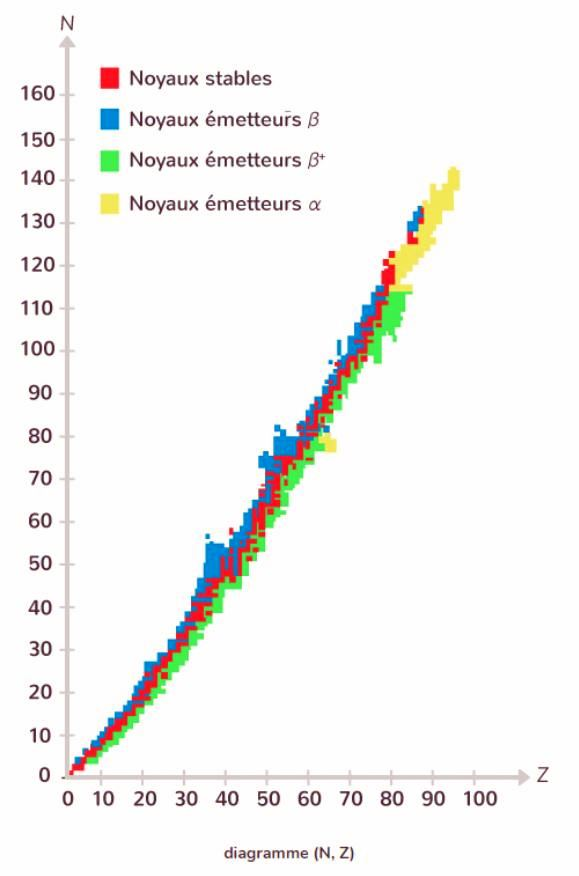
\includegraphics[width=0.95\linewidth]{imgs/p8/radioactivitynoyau.jpg}
\caption{Diagramme de Segré}
\label{fig:segré}
\end{wrapfigure}

La radioactivité des atomes est une conséquence de leur stabilité ... ou plutôt instabilité. Pour rappel, un noyau atomique est composé de protons et de neutrons, entouré d'un nuage d'électron. Les bretons sont positivement charger tandis que les autres ont donc pas de charges électriques. Par conséquent il faut l'existence d'une force supplémentaire pour Surmonter la répulsion électrostatique entre les protons dans le noyau. Cette force s'appelle l'\textbf{interaction forte}\eng{the strong force}, car elle existe seulement à l'échelle du noyau, et c'est l'interaction la plus forte entre les quatre interactions fondamentales.

L'interaction forte existe entre les protons et les neutrons. Nous pouvons imaginer l'interaction forte comme une sorte de colle qui existe seulement entre les protons et les neutrons. S'il y'a \textbf{trop de protons} dans le noyau, alors la répulsion électrostatique va dominer et le noyau se désintègre, tandis que si les \textbf{neutrons sont trop nombreux} dans le noyau il n'y a pas assez de interaction forte pour garder la cohésion du noyau; et donc il reste seulement une fine gamme de proportions les protons et de neutrons qui donne la stabilité maximale au noyau atomique. Cette ``\textbf{vallée de stabilité}'' est la où se trouvent les isotopes naturels, bien illustré dans le \textbf{diagramme de Segré} (c.f. Fig \ref{fig:segré}). 

\subsection*{Diagramme $(Z ; N)$}

La diagramme de Segré est un exemple d'un diagramme $(Z;N)$.  Ce type de diagramme vous permet non seulement de repérer les différents isotopes, mais permet aussi de visualiser les différentes types de transformations nucléaires, comme nous verrons dans les parties suivantes. 

Si l'on regarde sur le diagramme de Segré, nous voyons clairement une tranche d'isotopes stable, ou les proportions de neutrons et de protons sont telles que le noyau possède une cohésion durable: ce sont les isotopes de ces éléments que nous trouvons en abondance dans la nature. Les autres isotopes que nous trouvons en dehors de cette vallée de stabilité sont les isotopes instables, et donc susceptible à se désintégrer spontanément. 

L'élément 83, le bismuth, est considéré comme le dernier élément naturel avec un isotope stable. Tout élément de $Z>83$ n'a aucun isotope stable. Finalement, l'uranium ($Z=92$) est le dernier élément qui se trouve naturellement sur Terre, tout élément $Z>92$ sont produits artificiellement dans des laboratoires. 

\subsection{Écriture d'une réaction nucléaire}

Afin de mieux étudier les transformations nucléaires, il faut développer une façon de les écrire et de les modéliser. Nous allons donc réutiliser la notation utilisée précédemment pour modéliser les noyaux atomiques. 

Toutefois il faut d'abord comprendre que la modélisation correcte de ces transformations dépend de deux lois de conservation : 
\begin{itemize}
    \item \textbf{Conservation de la masse} : Dans le cas des noyaux atomiques, ceci implique la \textbf{conservation du nombre de masse $A$}. 
    \item \textbf{Conservation de la charge} : Dans le cas des noyaux atomiques, ceci implique la \textbf{conservation du numéro atomique $Z$}. 
\end{itemize}

Considérons les éléments chimiques \ce{^{A}_{Z}W}, \ce{^{A'}_{Z'}X} , \ce{^{A''}_{Z''}Y} 
\begin{itemize}
    \item Pour noter une transformation nucléaire on utiliser une flèche $\longrightarrow$. e.g. : 
    $$\ce{^{A}_{Z}W} \longrightarrow \ce{^{A'}_{Z'}X} + \ce{^{A''}_{Z''}Y}$$
    \item la \textbf{conservation de masse} implique : $A = A' + A'' $
    \item la \textbf{conservation de charge} implique : $Z = Z' + Z''$
    \item de manière générale la somme des $A$ avant la flèche doit égaliser la somme des $A$ après la flèche. De même pour les numéros de charge $Z$. 
\end{itemize}

De manière générale alors : 

\textbf{Une désintagration : }  $\ce{^{A}_{Z}W} \longrightarrow \ce{^{A'}_{Z'}X} + \ce{^{A''}_{Z''}Y} \quad \text{avec}\quad
\begin{cases}
A = A' + A'' \\
Z = Z' + Z''
\end{cases}
$

\textbf{Une fusion : } $\ce{^{A}_{Z}W} + \ce{^{A'}_{Z'}X}  \longrightarrow \ce{^{A''}_{Z''}Y} \quad \text{avec}\quad
\begin{cases}
A + A' = A'' \\
Z + Z' = Z''
\end{cases}
$

\textbf{Une fission :} $\ce{^{A}_{Z}W} \longrightarrow \ce{^{A'}_{Z'}X} + \ce{^{A''}_{Z''}Y} \quad \text{avec}\quad
\begin{cases}
A = A' + A'' \\
Z = Z' + Z''
\end{cases}$

\subsection{La radioactivité}

\begin{defn}{radioactivité}
\begin{itemize}
    \item La radioactivité est le phénomène associé à la \textbf{désintégration spontanée des noyaux instables}.
    \item Chaque noyau instable, dis radioactif, se désintègre \textbf{inéluctablement à un instant imprévisible}.
    \item Un noyau instable susceptible de se désintégrer s'appelle un \textbf{radionucléide}
    \item Un \textbf{radioisotope} est un isotope instable, susceptible de se désintégrer spontanément. 
    \item En raison de la radioactivité, un élément chimique peut se transformer en d'autres éléments.    
    \item Le noyau instable du départ s'appelle le \textbf{noyau ``père''}, et le noyau issue de la transformation est le \textbf{noyau ``fils''}. 
\end{itemize}
\end{defn}

En fonction de la raison de l'instabilité d'un isotope, il existe 3 catégories de radioactivité : 
\begin{itemize}
    \item Radioactivité $\alpha$
    \item Radioactivité $\beta^-$
    \item Radioactivité $\beta^+$
\end{itemize}

\subsubsection{Radioactivité $\alpha$}

La radioactivité alpha est due à un \textbf{excès de nucléons}. Elle affecte les noyaux situés sur les bords droit et au-delà de la vallée de stabilité du diagramme de Segré.

La radioactivité alpha comprend l'émission d'un noyau d'hélium $\ce{^4_2He}$ appelée une \textbf{particule alpha}.  L'équation générale de cette transformation est : 
\[\ce{^A_ZX -> ^{A-4}_{Z-2}Y + ^4_2He}\]

En traversant la matière, cette particule interagit principalement avec le cortège électronique des atomes du matériau traversé, ce qui les \textbf{excite} ou les \textbf{ionise}, mais seulement sur une très courte distance. Ce type de rayonnement a un pouvoir de pénétration plutôt faible (la peau humaine, ou une simple feuille de papier ou 4 à 5 cm d'air les arrêtent totalement).

\subsubsection{Radioactivité $\beta^-$}
La radioactivité bêta moins affecte les \textbf{noyaux qui possède un excès de neutrons} par rapport aux protons. Ils sont situés à gauche de la vallée de stabilité.
 
La radioactivité $\beta^-$ est la transformation d'un neutron en proton dans le noyau accompagné d'émission d'un électron et d'un anti-neutrino électronique. (L'explication de cette transformation de neutron en proton, est due à la $4^e$ interaction de la nature, l'interaction faible\eng{weak force}). Cette transformation est dite \textbf{isobarique} car il y a une \textbf{conservation de nombre de masse} $A$.

L'équation générale de cette transformation est : 
\[\ce{^A_ZX -> ^{A}_{Z+1}Y + ^0_{-1}e-}\]

Ce rayonnment (un électron) a une portée supérieure à celle d'une particule alpha, cependant une feuille d'aluminium peut l'arrêter. Cependant ce rayonnement interagit avec la matière en provoquant des excitations et des ionisations par diffusion. Le parcours des électrons dans la matière est plus important que celui des particules alpha (de l'ordre de quelques mètres maximum dans l'air). 

\subsubsection{Radioactivité $\beta^+$}
La radioactivité bêta moins affecte les \textbf{noyaux qui possède un excès de protons} par rapport aux neutrons. Ils sont situés à droite de la vallée de stabilité.
 
La radioactivité $\beta^+$ est la transformation d'un neutron en proton dans le noyau accompagné d'émission d'un positron (partenaire anti-matière de l'électron noté $\ce{e+}$ et d'un neutrino électronique (comme dans le cas du rayonnement $\beta-$, cette transformation est due à l'interaction faible). Cette transformation est isobarique. 

L'équation générale de cette transformation est : 
\[\ce{^A_ZX -> ^{A}_{Z-1}Y + ^0_{1}e+}\]

Il s'agit ici d'un rayonnement qui interagit, après avoir été ralenti, avec un électron du milieu provoquant son annihilation (conversion totale de la matière en énergie lors d'une rencontre entre une particule de matière et d'antimatière) et la production de deux rayons gamma de $511\; keV$ chacun.

\begin{figure}[H]
\centering
\begin{subfigure}{.26\textwidth}
  \centering
  % include first image
  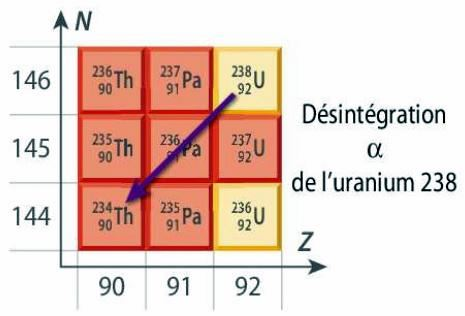
\includegraphics[width=.95\linewidth]{imgs/p8/alpha.jpg}  
\end{subfigure}
\begin{subfigure}{.26\textwidth}
  \centering
  % include first image
  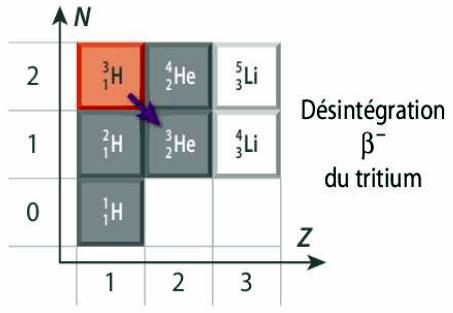
\includegraphics[width=.95\linewidth]{imgs/p8/beta-.jpg}  
\end{subfigure}
\begin{subfigure}{.26\textwidth}
  \centering
  % include first image
  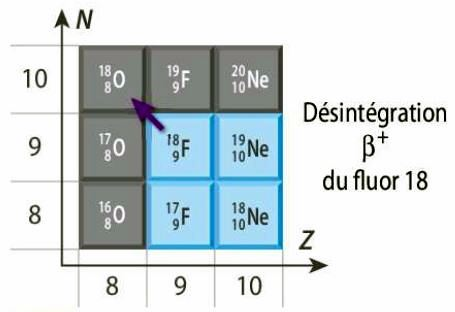
\includegraphics[width=.95\linewidth]{imgs/p8/beta+.jpg}  
\end{subfigure}
\begin{subfigure}{.17\textwidth}
  \centering
  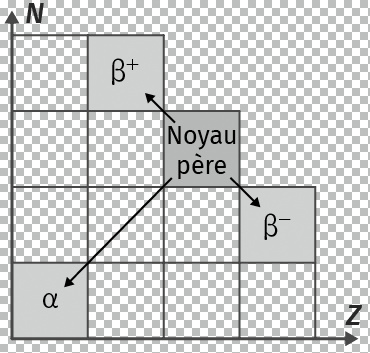
\includegraphics[width=.95\linewidth]{imgs/p8/desintegrations.jpg}  
\end{subfigure}
\caption{Les différents types de radioactivité sur un diagramme $(Z;N)$}
\end{figure}

\begin{rmrq}
% \begin{wrapfigure}[11]{r}{0.5\textwidth}
% \centering
% 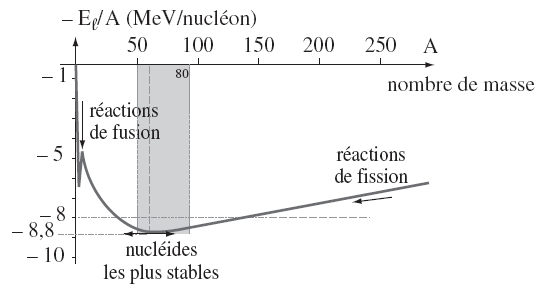
\includegraphics[width=0.95\linewidth]{imgs/p8/aston.jpg}
% \caption{La courbe d'Aston}
% \end{wrapfigure}
La courbe de la figure \ref{fig:aston} permet de comparer la stabilité des différents types de noyaux.
Sur cette figure, le niveau zéro de l’énergie correspond aux nucléons séparés et au repos. Un minimum de la courbe correspond une stabilité maximale. Les éléments à gauche de la zone de stabilité, y arrivent par fusion nucléaire, tandis que les élément plus lourds y arrivent par la fission. L'élément le plus stable est le fer. Parmi les nombreuse applications de cette courbe, est l'explication de l'évolution de la fusion au sein des étoiles vers l'élément fer avant de subir une nova ou supernova.
\begin{figure}[H]
\centering
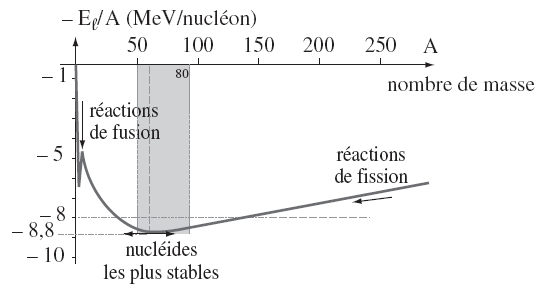
\includegraphics[width=0.85\linewidth]{imgs/p8/aston.jpg}
\caption{La courbe d'Aston}
\label{fig:aston}
\end{figure}
\end{rmrq}


\subsubsection{Rayonnement $\gamma$}
Les désintégrations nucléaires sont presque toujours accompagnées d'une émission électromagnétique de très haute énergie. Ceci est le cas car le noyau fils produit est souvent dans un état excité, c'est à dire à un niveau d'énergie supérieur à l'état fondamental. 

\begin{rmrq}
N'étant pas du à un déséquilibre baryonique, mais plutôt d'une excitation de l'atome, le rayonnement $\gamma$ est des photons, très énergétique et très pénétrant, qui nécessite beaucoup plus pour arrêter, 1-5 cm de plomb. 

En général, l'émission de rayons $\gamma$ suit une désintégration $\alpha$ ou $\beta$, car elle correspond à un ré-arrangement des nucléons, et notamment à une réorganisation de la charge électrique à l'intérieur du nouveau noyau.

En traversant la matière, il provoque trois types d'interactions :
l'effet photoélectrique ; la création de paires ; l'effet Compton.
\end{rmrq}

\begin{exo}
Le phosphore 30 et radioactif $\beta+$. Le noyau fils obtenu est dans un état excité :  il retrouve spontanément sur l'état fondamental en émettant un rayonnement $\gamma$.
\begin{enumerate}
    \item Écrire le symbole du noyau de phosphore 30.
    \item À quel élément chimique appartient le noyau fils obtenu?
    \item Indiquer l'équation de désintégration du phosphore 30.
    \item Écrire l'équation de l'émission $\gamma $ qui s'en suit.
\end{enumerate}
\vspace{5.5cm}
\end{exo}

\subsection{Rayonnement ionisant}


\section{Évolution temporelle d'une population radioactive}

Même si le comportement d'un seul noyau instable est absolument imprévisible, avec un assez grand nombre de noyaux, le comportement devient parfaitement modélisable (comme c'est souvent le cas avec des modèles probabilistes dépendant d'un grand nombre d'entité dans l'échantillon). Commençons alors par une définition importante : l'activité radioactive. 

\subsection{Loi de décroissance radioactive}

\begin{defn}{Activté radioactive\eng{Total activity}}
\begin{itemize}
    \item L'\textbf{activité} mesure le \textbf{nombre de désintégration} radioactive qui se produisent dans un échantillon.
    \item l'activité est noté $A$ et se mesure en \textit{Bequerel} noté $Bq = s^{-1}$. 
    \item Un $Bq$ est une désintégration par seconde. 
\end{itemize}
\end{defn}

Pour un échantillon contenant $N$ radionucléides, l'activité $A(t)$ est donnée par : \[ A(t) = - \diff{N}{t} \]

Naturellement, $A(t)$ est proportionnelle au nombre $N$ de radionucléides : $A \propto N$. Nous avons donc 
\begin{align*}
    A(t) = - \diff{N}{t} &  \propto N \\
    \diff{N}{t} &= -\lambda \cdot N \tag{1}
\end{align*}

\begin{wrapfigure}{r}{0.28\textwidth}
\centering
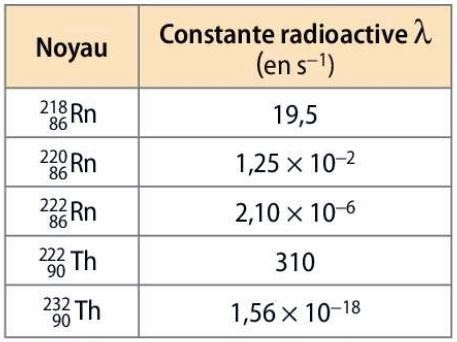
\includegraphics[width=0.95\linewidth]{imgs/p8/lambdatable.jpg}
\caption{Quelques constantes radioactives}
\end{wrapfigure}

La constante de proportionnalité $\lambda$ s'appelle la \textbf{constante radioactive} du radionucléide, est une propriété du noyau, est s'exprime en $s^{-1}$ (car c'est une mesure de nombre de désintégration par seconde).  Vous connaissez bien maintenant les relations de forme (1), il s'agit bien d'une équation différentielle de premier ordre. Par conséquent, pour une population initiale de $N(0) = N_0$ la solution de (1) est : 

\[ N(t) = N_0 e^{-\lambda t}\]

et 

\[ A(t) = A_0 e^{-\lambda t} \quad \text{ avec }\quad A_0 = \lambda N_0\]

Nous voyons donc, sans beaucoup d'étonnement, que l'activité suit une loi de \textbf{décroissance exponentielle}, un fait que nous allons exploiter dans la partie suivante.

\begin{rmrq}
Voici une démonstration de cette relation en plus de détail, à partir d'un raisonnement probabiliste. 

Considérons un échantillon contenant à nombre $\Delta N$ de noyaux radioactifs un instant $t$ donné. Pendant la durée $\Delta t$, le nombre de noyaux radioactifs diminue et passe de $N$ à $N+\Delta N$, avec $\Delta N<0$. Il y a donc eu désintégration de $-\Delta N$ noyaux. 

La probabilité $P$ pour que $-\Delta N$ noyaux se désintègrent pendant la durée $\Dt$ est : $P = \dfrac{|\Delta N|}{ N}= -\dfrac{\Delta N}{N}$. Cette probabilité est proportionnelle à la durée $\Dt$ : $P =- \dfrac{\Delta N}{N} = \lambda\Dt$.

Le reste est comme avant : dans la limite où $\Dt \rightarrow 0$, nous avons $ - \dfrac{\dl N}{N} = \lambda\dl t $ et prenant l'intégral des deux cotés (avec conditions initiales $N(t=0) = N_0$ : 
\[\int \dfrac{\dl N}{N} = - \int \lambda\dl t \]
dont la solution : 
\[ \ln{N(t)} = -\lambda t + k \]
$k$ est la constante d'intégration qui nous permet, en utilisant les conditions initiales de trouver la solution : 
\[N(t) = N_0e^{-\lambda t}\]
\end{rmrq}

\newpage
\subsection{Demi-vie \& constante du temps}

\begin{wrapfigure}[7]{r}{0.33\textwidth}
\centering
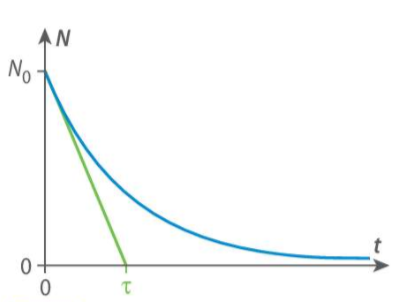
\includegraphics[width=0.95\linewidth]{imgs/p8/decroit.png}

\end{wrapfigure}

Comme toute décroissance exponentielle, il y a une constante de temps qui nous permet de déterminer la vitesse de la décroissance, et ici, par conséquent, une mesure de la radioactivité. 

En suivant le comportement d'une fonction exponentielle, nous voyons que la constante de désintégration $\lambda$ permet de définir un temps caractéristique de l'échantillon radioactif considéré, appelé constante de temps. La constante de temps, noté $\tau$, est définie par la relation :

\[ \tau = \dfrac{1}{\lambda}\]

Comme nous avons déjà vu dans le cas de l'étude des vitesse des réactions, ou de la charge/décharge d'un condensateur (et tout autre cas ou un comportement peut être modélisé par une fonction exponentielle), une mesure couramment utilisée est le temps qu'il faut pour que la grandeur étudiée atteigne la moitié de sa valeur initiale.  Dans le cas de la décroissance nucléaire on parle de \textit{la demi-vie}.

\begin{defn}{Demi-vie \eng{half-life}}
\begin{itemize}
    \item La demi-vie est la durée nécessaire pour que la moitié de l'échantillon radioactif se désintègre.
    \item Après \textit{une} demi-vie il reste la moitié de la quantité initiale. 
    \item La demi-vie s'exprime $t_{\nicefrac{1}{2}} = \dfrac{\ln{2}}{\lambda}$
\end{itemize}
\end{defn}

\begin{figure}[H]
\centering
\begin{subfigure}{.32\textwidth}
  \centering
  % include first image
  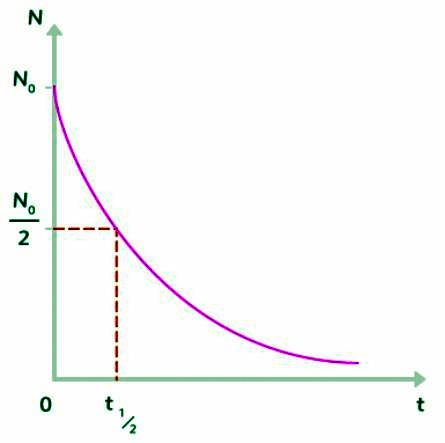
\includegraphics[width=.95\linewidth]{imgs/p8/demivie.jpg}  
\end{subfigure}
\begin{subfigure}{.32\textwidth}
  \centering
  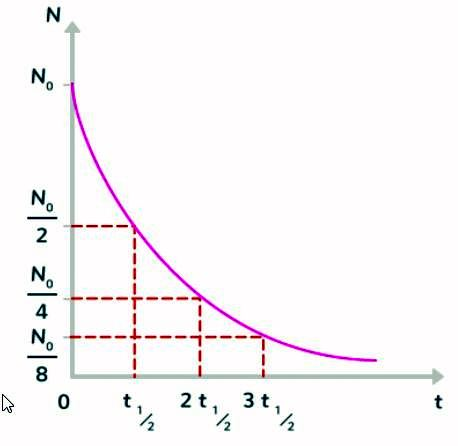
\includegraphics[width=.95\linewidth]{imgs/p8/decroissances.jpg}  
\end{subfigure}
\begin{subfigure}{.32\textwidth}
  \centering
  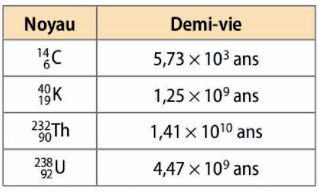
\includegraphics[width=.95\linewidth]{imgs/p8/demiviesexe.jpg}  
\end{subfigure}
\caption{Évolution des nombres d'isotopes dans un échantillon .}
\end{figure}

\begin{exo}
Démontrer $t_{\nicefrac{1}{2}} = \dfrac{\ln{2}}{\lambda}$ à partir de la définition de la demi-vie. 
\vspace{4cm}
\end{exo}

\begin{exo}
Une source de thorium-90 composée à un instant $t_0$ d'un nombre $N_0 = 2,66\es{18}$ atomes radioactifs révèle une activité $A_0 = 1,14\es{14}\;Bq$. 
\begin{enumerate}
    \item Calculer la constante d'intégration du thorium 90. 
    \item En déduire sa constante de temps $\tau$, puis sa demi-vie $t_{\nicefrac{1}{2}}$.  Exprimer dans l'unité de temps la mieux adaptée.
    \item Calculer le nombre de noyaux radioactifs restant dans la source 100 jours plus tard, puis 1000 jours plus tard.
\end{enumerate}
\vspace{5cm}
\end{exo}




\section{Radioactivité naturelle \& applications}  

Malgré nos peurs en ce qui concerne la radioactivité, la nature est radioactive. Il y a de la radioactivité naturelle tout autour de nous, dans la croûte terrestre, et ailleurs. Il existe plusieurs source de radioactivité naturelle sur terre : 
\begingroup
\begin{wrapfigure}{l}{0.45\textwidth}
\centering
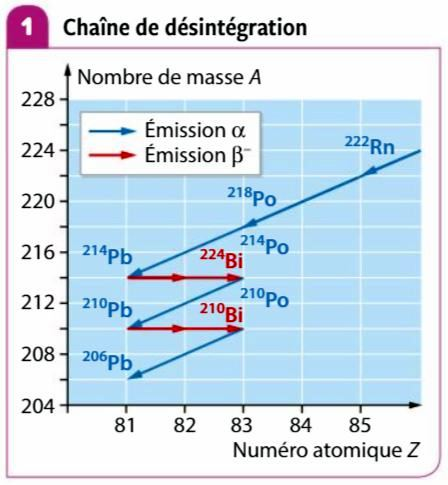
\includegraphics[width=0.95\linewidth]{imgs/p8/chainedesinteg.jpg}
\end{wrapfigure}
\begin{itemize}
    \item Les noyaux radioactifs présents depuis la formation de la terre dans la croûte terrestre pour qu'une partie subsiste même aujourd'hui. Par exemple le potassium-40 ou encore l'uranium-235 ou 238.
    \item Les noyaux radioactifs de période plus courte voir très courte. Ces noyaux sont souvent des noyaux fils des atomes instables de demi-vies de longues durées.  Il s'agit souvent des chaînes de désintégration en cascade comme dans la figure ci-contre. On obtient ainsi une série de désintégrations jusqu'à un noyau stable. L'ensemble des noyaux radioactifs qui apparaissent au cours de ces différents désintégration la question constitue une \textbf{famille radioactive}.
    \item Les noyaux radioactifs formés dans l'atmosphère, par action des rayonnements cosmiques sur certains atomes. Les plus importants sont le tritium (hydrogène-3) et le carbone-14.
\end{itemize}
\endgroup

\begin{figure}[h]
\centering
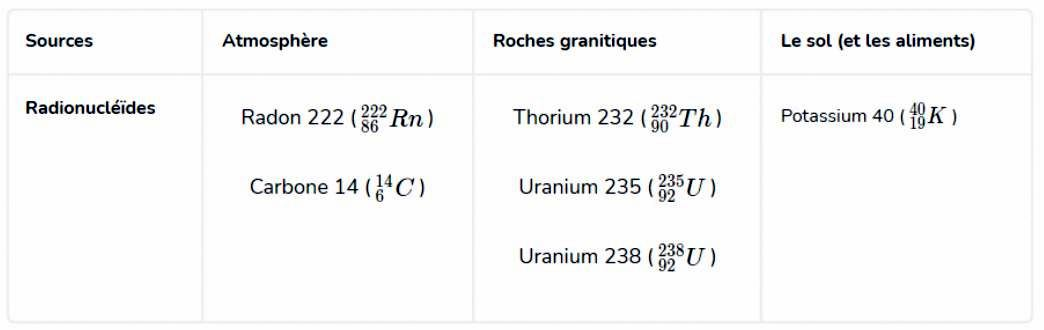
\includegraphics[width=0.75\linewidth]{imgs/p8/nautreradio.jpg}
\end{figure}

Il y a un certain nombre d'éléments radioactifs qui sont artificiellement produit dans les laboratoires ou dans les centrales nucléaire ou dans des accélérateurs de particules. Tout élément chimique au-delà de l'élément 92, c'est-à-dire l'uranium, son artificiellement produits et ne se trouvent pas spontanément dans la nature.

\subsection{Datation}

\begin{wrapfigure}[15]{r}{0.5\textwidth}
\centering
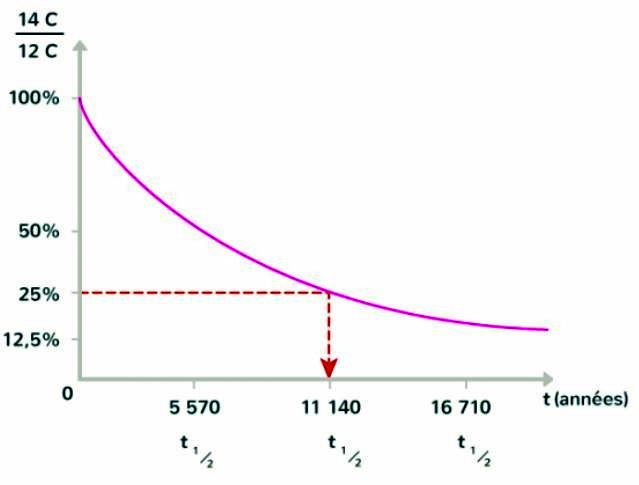
\includegraphics[width=0.95\linewidth]{imgs/p8/datation.jpg}
\caption{Exemple de datation carbone-14}
\end{wrapfigure} 
De loin, l'application la plus connu des propriétés radioactives de la matière est la datation au carbone-14, exploitée dans beaucoup de domaines des sciences, de la biologie jusqu'à l'archéologie.

La proportion de l'isotope carbone-14, avec une demi-vie d'environs 5680 ans, est très faible ($ \sim 10^{-12}$) mais à peu près constante au cours du temps. Tout organisme vivant échangeant du carbone avec l'atmosphère fixe l'élément carbone par les tissus renfermant la même proportion d'isotope carbone-14 que l'atmosphère. Cette proportion est donc constante tout au long de la vie de l'organisme. A leur mort les organismes cessent  d'échanger l'élément carbone, par conséquent le carbone-14 n'est plus régénéré, et sa quantité diminue selon la loi de décroissance radioactive.

La quantité de carbone-14 restant dans un échantillon et mesurable jusqu'à l'âge d'environ 50 000 ans. Pour dater des événements plus anciens donc, il existe d'autre méthode d'utilisation du noyau radioactif avec des demi-vies plus longues, comme le potassium-40 où le thorium-232.

\end{document}